% !TeX spellcheck = sk_SK-Slovak
\documentclass[a4paper]{article}
\usepackage[slovak]{babel}
\usepackage[utf8]{inputenc}
\usepackage[T1]{fontenc}
\usepackage{a4wide}
\usepackage{amsmath}
\usepackage{amsfonts}
\usepackage{amsthm,amssymb}
\usepackage{mathrsfs}
\usepackage[small,bf]{caption}
\usepackage{subcaption}
\usepackage{xcolor}
\usepackage{graphicx}
\usepackage{enumerate}
\usepackage{hyperref}
\usepackage[a4paper, total={7in, 10.2in}]{geometry}

\let\origfontsize\fontsize
\def\fontsize#1#2{\origfontsize{11}{14.5}}


\pagestyle{empty}
\setlength{\parindent}{0pt}

\newenvironment{modenumerate}
{\enumerate\setupmodenumerate}
{\endenumerate}

%\renewcommand{\thesubsection}{\thesection.\alph{subsection}}
%\renewcommand{\thesubsection}{\alph{subsection})}
\renewcommand{\thesection}{}
\renewcommand{\thesubsection}{}
\renewcommand{\thesubsubsection}{}

\begin{document} 
	
	\pagenumbering{arabic}
	\pagestyle{plain}
	
	\begin{center}
		\sc\large
		PHYSICAL BASED ANIMATIONS AND MATHEMATICAL MODELING
		\\
		SKUSKA
	\end{center}
	
	Autor: Marián Kravec
	\\
	
	\section{Set A}

	Pri postupe animovanie "Skeleton and skinning" sa najskôr modeluje kostra modelu (zväčša nejakej postavičky) a následne sa na túto kostru modeluje koža. Celý proces má dve časti:
	\begin{itemize}
		\item Rigging Skeleton - ide o proces pri ktorom sa vytvára hierarchická kostra objektu, keďže táto kostra je hierarchická tak okrem informácie ako je pozícia, rotácia a dĺžka kosti určujeme aj informáciu o rodičovskej kosti (výnimkou je koreňová kosť) a detských kostiach (v slovenčine to znie strašne), kosti sa navzájom prepájajú na koncoch kde vytvárajú kĺby pre ktoré sa definujú limity pohybu 
		\item Skinning skeleton - proces pri ktorom sa na kostru aplikuje koža, zväčša definovanú ako sieť bodov (vrcholov), kde pre každý bod (vrchol) definuje množinu váh hovoriacej o príslušnosti daného bodu (vrcholu) k blízkym kostiam 
	\end{itemize}
	
	Samotná animácia následne funguje tak, že animujeme iba pohyb kostry a pozície bodov (vrcholov) siete kože je nakoniec prepočítaný na základe novej pozície kostí.
	
	\section{Set B}
	\centerline{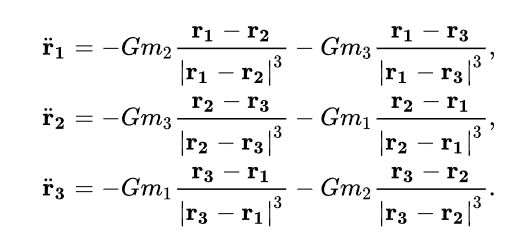
\includegraphics[width=0.6\textwidth]{rovnice}}
	\subsection{1.}
	\subsubsection{a)}
	Keďže som sa narodil 18.9. tak hodnoty $MM=9$ a $DD=18$, ak si za zvyšné hodnoty počiatočných parametrov bodov zvolíme 0 naše body sa na počiatku nachádzajú:
	\begin{align*}
		r_1=\{MM, 0,DD\} = \{9,0,18\}\\
		r_2=\{DD,MM, 0\}= \{18, 9,0\}\\
		r_3=\{0, DD, MM\}= \{0,18,9\}
	\end{align*}
	
	\subsubsection{b)}
	Keďže nemáme tušenie ako sa systém bude správať hodnoty počiatočných derivácii určíme pomerne náhodne:
	
	\begin{align*}
		r'_1=\{0.5,0.1,0.1\}\\
		r'_2=\{0.1,0.5,0.1\}\\
		r'_3=\{0.1,0.1,0.5\}
	\end{align*}
	
	(ako bolo spomínané druhé derivácie nepotrebujú určiť počiatočnú podmienku ale nič nám nebráni ich všetky nastaviť na 1 a nikdy nepoužiť)
	
	\subsubsection{c)}
	
	Ešte posledné konštanty a to sú $G=6.674*10^(-11)$ a hmotnosti ktoré si na začiatok zadajme takto $m_1= 10^11$, $m_2=10^11$, $m_3=10^11$.
	\\
	
	Ak si naše počiatočné body vykreslíme dostaneme takýto výsledok:
	
	\centerline{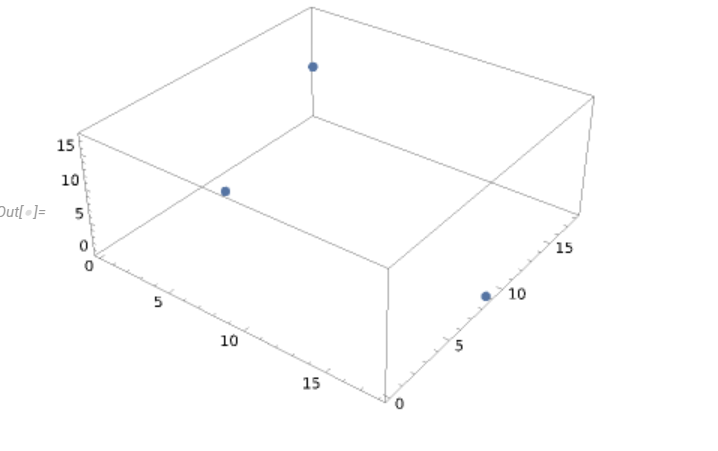
\includegraphics[width=0.6\textwidth]{pociatok}}
	
	\subsection{2.}
	
	Teraz môžeme začať s samotným modelovaním pohybu troch telies.
	
	Najskôr si zapíšeme rovnice a počiatočné podmienky:
	
	\centerline{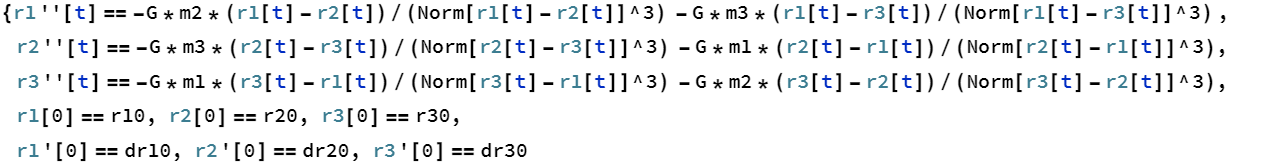
\includegraphics[width=0.6\textwidth]{rovnice_2}}
	
	\subsubsection{a)}
	A nastavíme metódu na numerické integrovanie na Runge-Kutta metódu (použijeme metódu priamo ponúknutú Wolframom) konkrétne použijeme jej explicitnú verziu.
	
	\centerline{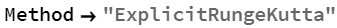
\includegraphics[width=0.4\textwidth]{method}}
	
	\subsubsection{b)}
	Najskôr si zapíšeme konštanty a počiatočné hodnoty:
	
	\centerline{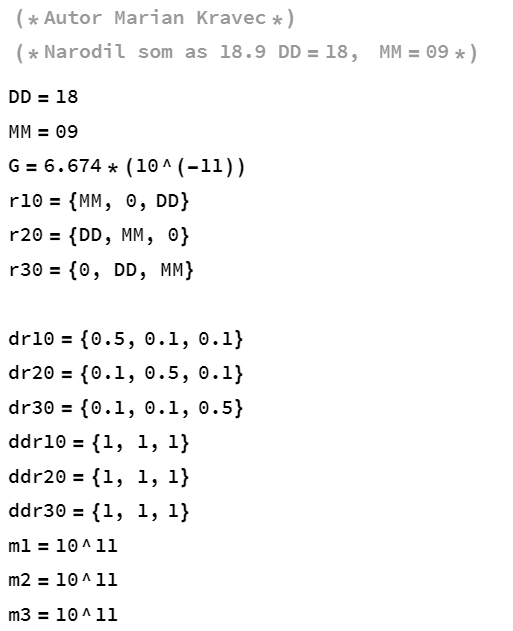
\includegraphics[width=0.3\textwidth]{hodnoty}}
	
	Ako ďalšie rovnice a počiatočné podmienky:
	
	\centerline{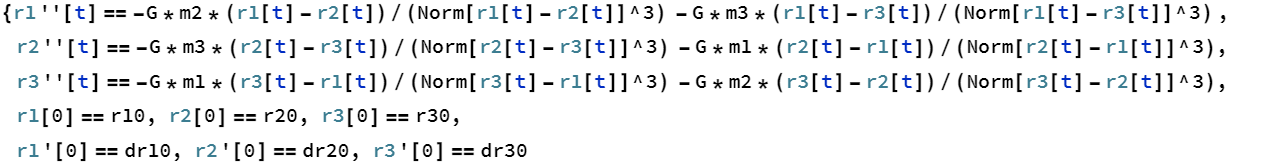
\includegraphics[width=0.8\textwidth]{rovnice_2}}
	
	A cele to poskladáme do funkcie na riešenie diferenciálnych rovníc:
	
	\centerline{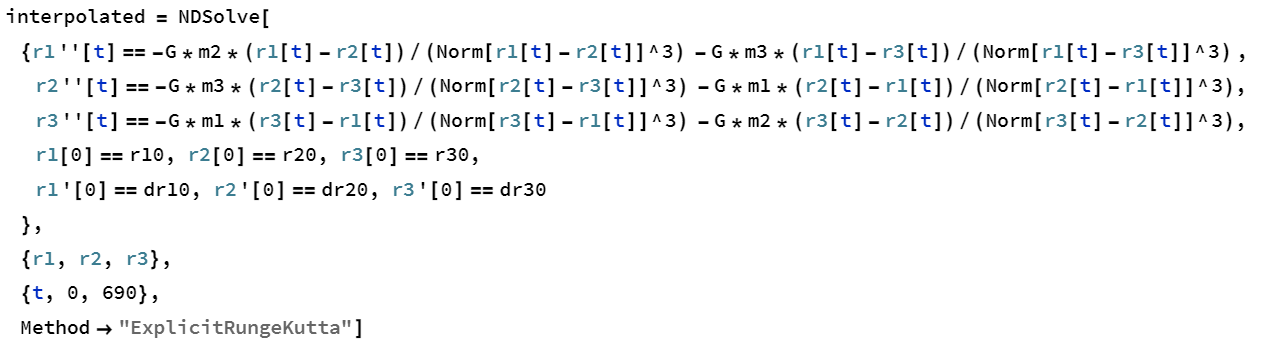
\includegraphics[width=0.8\textwidth]{ndsolve}}
	
	\subsubsection{c)}
	
	Aby sme s najväčšou pravdepodobnosťou videli pohyb budeme interpolovať prvých 100 sekúnd a rovnaký časový úsek vykreslíme v ďalšej časti.
	
	\subsubsection{d)}
	
	 Keď budeme modelovať systém s hodnotami zadanými v časti 1. prvých sto sekúnd a výsledok vykreslíme dostaneme takýto pohyb objektov:
	 
	 \centerline{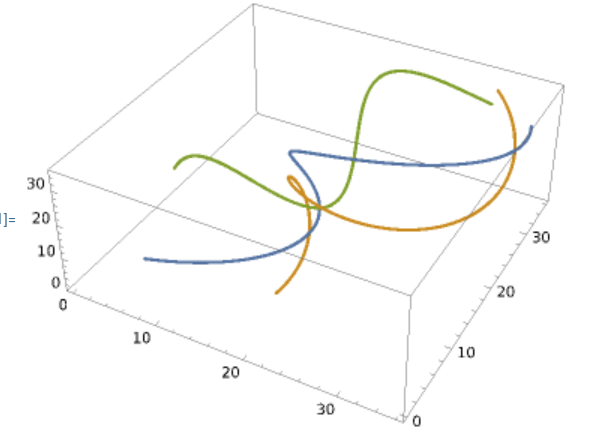
\includegraphics[width=0.4\textwidth]{pohyb_1}}
	 
	 Vidíme peknú interakciu medzi objektami.
	 
	 \subsubsection{e)}
	 
	 Teraz skúsme modelovanie zopakovať ale pre 690 sekúnd (po tomto čase začíname byť náš systém so súčasnými podmienkami tuhý a Wolfram to nevie modelovať):
	 
	 \centerline{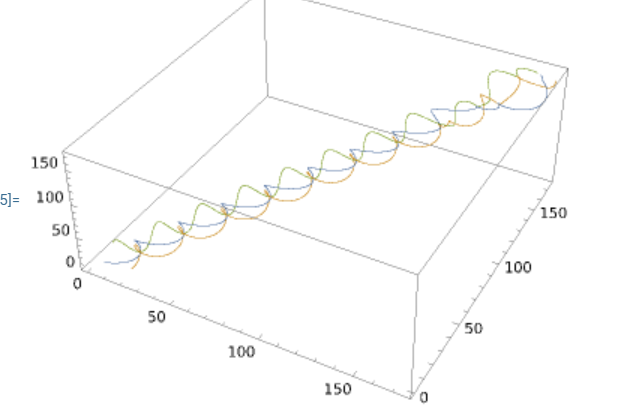
\includegraphics[width=0.8\textwidth]{pohyb_2}}
	 
	 Tu už lepšie vidíme správanie systému, kde si môžeme všimnúť že telesá idú spoločne špirálovitým pohybom jedným smerom, z počiatku to vyzerá, že ich pohyb by sa mohol považovať za periodický (opakuje sa rovnaký pattern) avšak ten sa kazí na konci, čo môže byť spôsobené buď tým, že systém nie je periodický a iba začiatok sa tak javí alebo tým, že chyba interpolácie je už príliš veľká a model už nezopakuje rovnakú periódu aj napriek tomu, že tam je. 
	
	\subsection{3.}
	
	\subsubsection{a)}
	
	Body umiestnime na trojuholník tak, že im všetkým dáme nulovú z súradnicu, prvý bod pošleme do počiatku súradnicovej sústavy, druhému dáme x-ovú súradnicu rovnú 3 a tretiemu y-ovú rovnú 4:
	
	\begin{align*}
		r_1=\{0,0,0\}\\
		r_2=\{3,0,0\}\\
		r_3=\{0,4,0\}
	\end{align*}
	
	Hodnoty počiatočných derivácii a hmotností nastavme takto (tieto hodnoty vznikli pomocou metódy pokus omyl aby sa systém nestal tuhým veľmi rýchlo).
	
	\begin{align*}
		r'_1=\{0.001,0.01,0.01\}\\
		r'_2=\{0.01,0.001,0.01\}\\
		r'_3=\{0.01,0.01,0.001\}\\
		m_1=5*10^7\\
		m_2=4*10^7\\
		m_3=3*10^7
	\end{align*}
	
	\subsubsection{b)}
	
	Ak tento systém budeme modelovať po dobu 1800 sekúnd, čiže 30 minút dostaneme takýto pohyb:
	
	\centerline{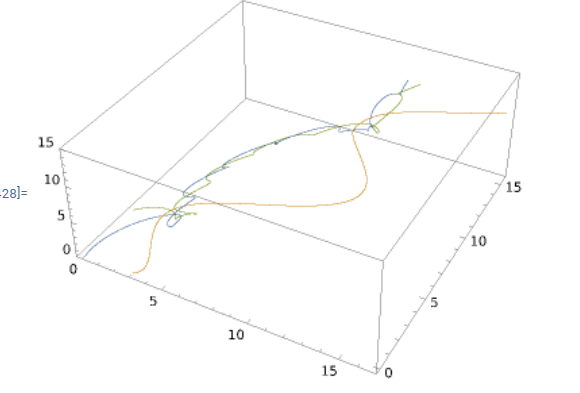
\includegraphics[width=0.8\textwidth]{pohyb_3}}
	
	Vidíme, že výrazne viac interagujú objekty 1 a 3 a objekt 2 je iba "ťahaný ich smerom" ale z môjho pohľadu to vyzerá na pomerne chaotické správanie.
	
	\subsubsection{c)}
	
	Začnime tým, že budeme robiť malá zmeny v hmotnosti telies (zmena od 0 po $10^4$ kg čo je pri ich hmotnosti ($10^7$) pomerne mála zmena).
	
	V druhom teste pridáme aj malé zmeny počiatočných derívacii (zmenu o maximálne 0.00001 pre každú hodnotu).
	
	\subsubsection{d)}
	
	Pri prvom teste zmeny iba hmotností:
	
	\centerline{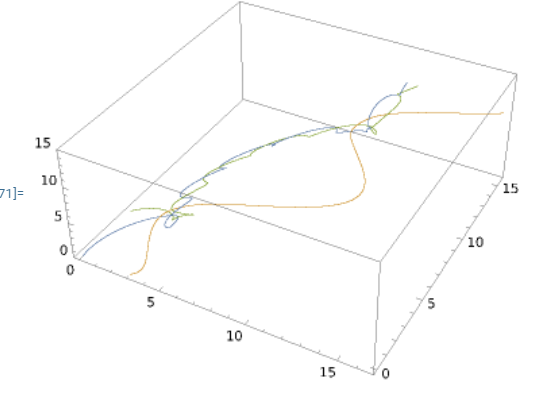
\includegraphics[width=0.8\textwidth]{pohyb_4}}
	
	Vidíme, že táto zmena nemá žiaden vplyv na pohyb telies, čiže pohyb stabilný pri malých zmenách hmotnosti. 
	\\
	
	Ak pridáme aj zmeny/chyby počiatočných derivácii:
	
	\centerline{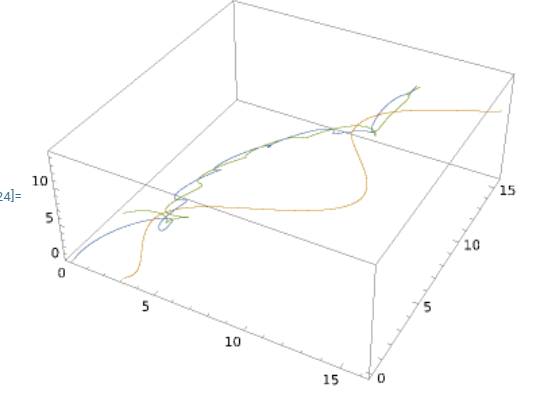
\includegraphics[width=0.8\textwidth]{pohyb_5}}
	
	Tu vidíme, že mierne zmeny sú viditeľné ale celkové správanie je stále stabilné.
	
	\subsubsection{e)}
	
	Skúsme, hodnoty chýb zväčšovať kým sa správanie zásadnejšie nezmení.
	\\
	
	V prípade hmotnosti sa systém ukazuje ako veľmi stabilný keďže na to aby sa zmenou hmotnosti jeho správanie zmenilo takto výrazne:
	
	\centerline{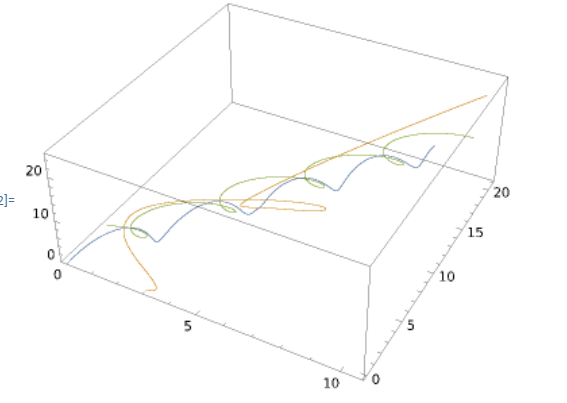
\includegraphics[width=0.8\textwidth]{pohyb_6}}
	
	Bolo potrebná aby zmena hmotnosti mohla byť až z intervalu od $0$ po $10^7$ kg. Konkrétne v ukážkovom prípade sa hmotnosť objektu 2 znížila len na približne tisícinu pôvodnej hmotnosti čo spôsobilo, že jeho vplyv na objekty 1 a 3 s výrazne väčšou hmotnosťou bola zanedbateľné a preto sa objekty 1 a 3 dostali do periodického pohybu ignorujúc objekt 2.
	\\ 
	
	V prípade zmien počiatočných podmienok tak stačí aby bola zmena z intervalu od $0$ po $0.001$ na to aby sa bežne stávalo, že sa správanie zmení napríklad na takéto:
	
	\centerline{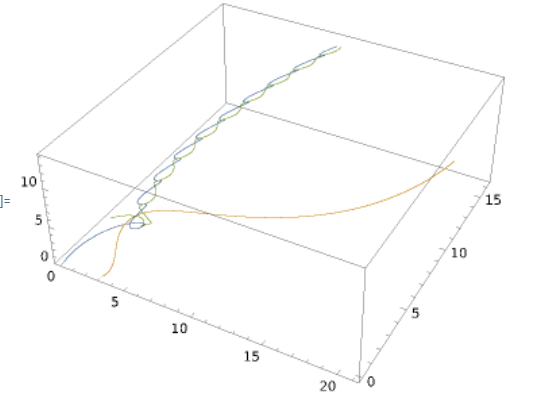
\includegraphics[width=0.8\textwidth]{pohyb_7}}
	
	Kde aj napriek tomu, že hmotnosť objektu 2 je porovnateľná s 1 a 3 nastane situácia, že sa tento objekt dostane príliš ďaleko a minimálne ovplyvňuje zvyšné 2 objekty ktoré sa znovu dostávajú do periodického pohybu.
	 
	\section{4.}
	
	\subsection{a)}
	
	Snaha bola nasimulovať takýto systém:
	
	\centerline{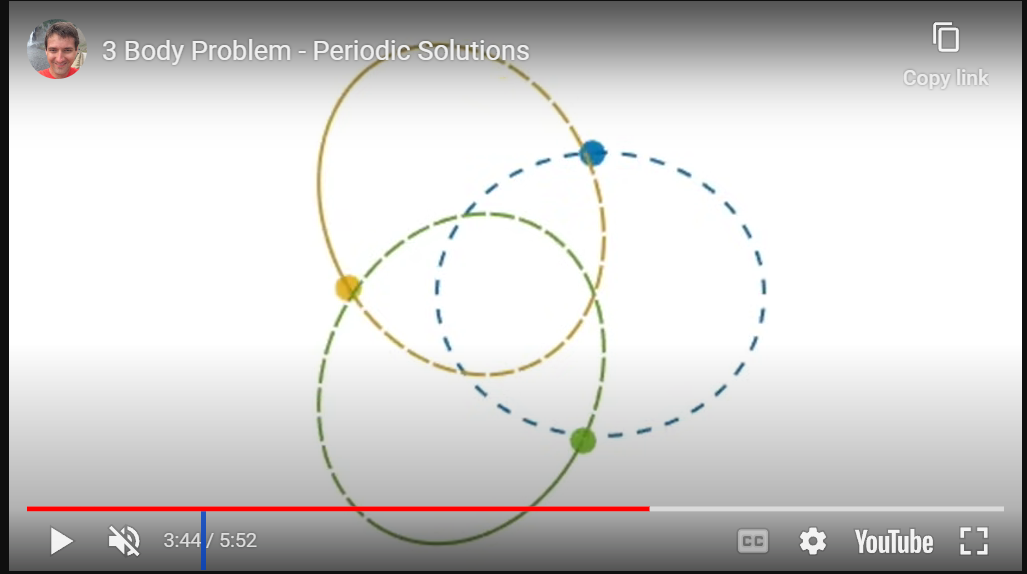
\includegraphics[width=0.8\textwidth]{system}}
	
	Ale kvôli časovým obmedzeniam sa to nepodarilo.
	
	Keď som nastavil parametre následovne:
	

	
	\begin{align*}
		r'_1=\{0.05*Sin[Pi/3],-0.05*Sin[Pi/6],0\}\\
		r'_2=\{0.05*Sin[Pi/6],0.05*Sin[Pi/3],0\}\\
		r'_3=\{-0.05,0,0\}\\
		m_1=10^9\\
		m_2=10^9\\
		m_3=10^9
	\end{align*}
	
	\subsubsection{b)}
	
	Tak počiatočné správanie vyzeralo sľubne:
	
	 \centerline{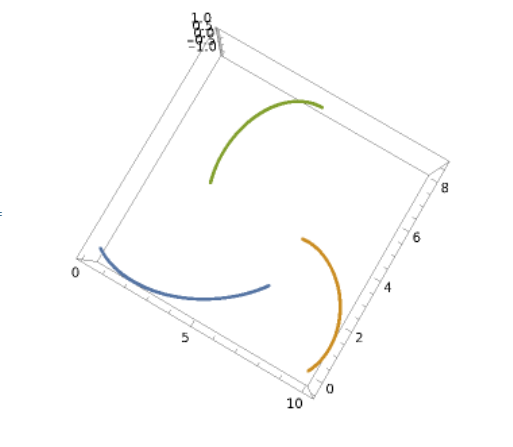
\includegraphics[width=0.8\textwidth]{pohyb_8}}
	
	A potom sa to celé rozbilo:
	
	\centerline{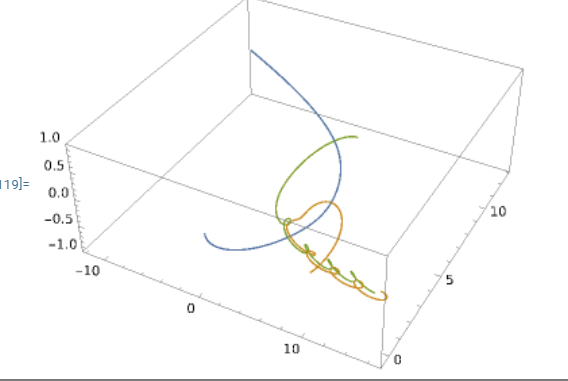
\includegraphics[width=0.8\textwidth]{pohyb_9}}
\end{document}